\chapter{Experiments and discussions}
\section{Experimental setup}\label{sec:setup}
% \subsection{Experimental environment}

\subsection{Configurations for market and client models}
For empirical evaluation, we consider the following market with two economy states $\mathcal Y=\{1,2\}$. $1$ is a bad economy and $2$ is a good one. Based on \citeA{chauvet2006dating}, we set the transition matrix for the economy states is given by $$P=\begin{bmatrix}
0.95 & 0.05\\
0.1 & 0.9
\end{bmatrix}$$ indicating that there's a high probability that the economy state stays the same but there's also positive probability to escape. The initial economy is set to be the bad one, i.e. $y_0=1$.

In the bad economy, the risk-free asset has zero return rate, while the risky asset has return drawn from $\mathcal N(0.01,0.05^2)$. In the good economy, the risk-free asset has a return rate of $0.01$ and the risky asset has return drawn from $\mathcal N(0.03, 0.1^2)$. Using the notations introduced in Section \ref{sec:market_model}, we have
    \begin{align*}
    r(y)=\begin{cases}0.00,&y=1\\
    0.01, & y=2
    \end{cases},\qquad
    \mu(y)=\begin{cases}0.01,&y=1\\
    0.03, & y=2
    \end{cases},\qquad
    \sigma(y)=\begin{cases}0.05,&y=1\\
    0.1, & y=2
    \end{cases}.\qquad
    \end{align*}

Unless otherwise specified, we set the time horizon $T$ to be $12$ and the interaction interval to be $3$, indicating a one-year robo-advising product with quarterly interactions.

As for the client, unless otherwise specified, we set the personalized parameters as follows\begin{align*}
    \gamma_0=4,\quad \alpha=0.01,\quad \beta=4,\quad p_\epsilon=0.05,\quad \sigma_\epsilon=0.64.
\end{align*}

Given the configuration for the market, client and the robo-advisor models, we run backwards induction as a one-time pre-processing step to find the optimal strategy at all timestamps given all possible states $\tilde d$. Then, for all the experiments we conduct, we simulate the market and run the robo-advising algorithm for an extensive number of trials and report the mean values for statistical significance.

\subsection{Implementation details}
We implement our robo-advising algorithm in Python\footnote{https://www.python.org/} and SciPy\footnote{https://scipy.org/} and run all experiments on Linux 20.04 LTS in a consumer-level machine equipped with Ryzen 9 5900HS and 32 GB of RAM. Our implementation follows Algorithm \ref{alg2} with approximation as described in Section \ref{sec:approx}. Although the algorithm has been described in great detail in Section \ref{sec:comp}, we specify the following important implementation details.

\subsubsection{Discretization configuration}
As suggested by Theorem \ref{thm:disc}, for each $n$, we need to evaluate the values of $\mu_n^a,\mu_n^{az},\mu_n^{bz},\mu_n^{bz^2},\tilde\pi_n^*,\allowbreak a_n,b_n$ given all possible states $\tilde d_n\in\tilde{\mathcal D}_n$. Therefore, we discretize the space $\tilde{\mathcal D}_n$:\begin{enumerate}
    \item For economy states at current time and the most recent interaction time, which is discrete, we naturally enumerate all the possible values in $\mathcal Y={1,2}$.
    \item For cumulative excess returns, we consider a range of $[-0.5,0.5]$ and discretize the range with a grid size of $0.1$.
    \item For risk aversion values, we consider a range of $(0,10]$ and discretize the range with a grid size of $0.5$.
\end{enumerate} This is a reasonable discretization grid because in our experiments, as the values almost never fall out of the specified ranges.

In backwards induction, for all $n$, we fill in the values of $\mu_n^a,\mu_n^{az},\mu_n^{bz},\mu_n^{bz^2},\tilde\pi_n^*,\allowbreak a_n,b_n$ at all grid points in $\tilde{\mathcal D}_n$. For querying data at states which are not a grid point, we use linear interpolation \cite{meijering2002chronology} to construct reasonable new data points from values at neighbor grid points. 

\subsubsection{Approximate integration over $\epsilon$}

Note that as pointed in the proof of Theorem \ref{thm:disc}, one need to integrate over the randomness of $\epsilon=\epsilon_{\tau_n+1}+\ldots+\epsilon_{n+1}$ whose distribution is a $\phi$-fold convolution of $\epsilon_n$ whose distribution is defined in Equation \eqref{eq:eps}. Note that this is not trivial to integrate because the probability density function for each $\epsilon_n$ is not continuous, i.e.$$f_{\epsilon_n}(x)=\begin{cases}
    \frac{p_\epsilon}{\sigma_\epsilon}\varphi\left(\frac{x}{\sigma_\epsilon}\right), \qquad &x\neq 0\\
    (1-p_\epsilon)+\frac{p_\epsilon}{\sigma_\epsilon\sqrt{2\pi}}, &x=0
\end{cases}$$ where $\varphi(\cdot)$ is the probability density function for the standard Gaussian $\mathcal N(0,1)$.

We take an approximation approach by first evenly taking many values from the range of $\epsilon_n$ and treat $\epsilon_n$ as a discrete random variable. We calculate the probability mass function for this approximate discrete random variable, and apply Fast Fourier Transform convolution to find the probability mass function for $\epsilon=\epsilon_{\tau_n+1}+\ldots+\epsilon_{n+1}$, and using the PMF to calculate the expectation over the randomness of (now discrete) $\epsilon$. Thus, we transform a difficult integration operation into a weighted sum. To be more specific, we evenly take $65$ points from $[-2,2]$ to form the discrete random variables.

\section{Optimal investment strategy}

\begin{figure}[t]
    \centering
    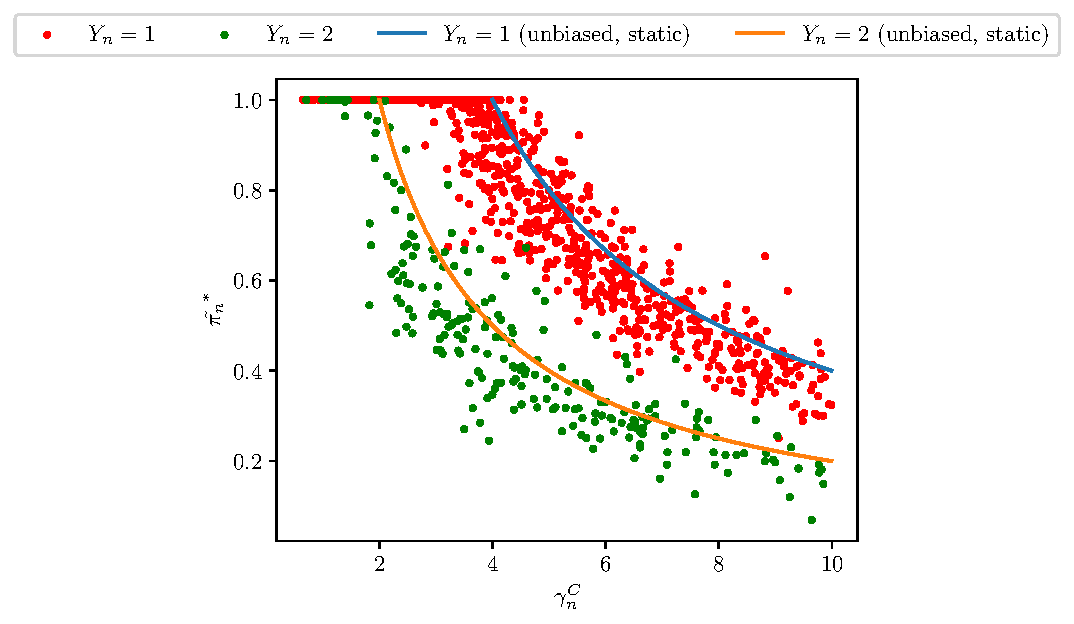
\includegraphics[width=\textwidth]{imgs/optimal_strategy.pdf}
    \caption{Optimal investment strategy as a function of client's risk aversion.}
    \label{fig:opt}
\end{figure}

Experimental configuration follows Section \ref{sec:setup}. We report in Figure \ref{fig:opt} the optimal proportion of wealth allocated to the risky asset, $\tilde\pi_n^d$, as a function of client's risk aversion, $\gamma_n^C$, prevailing six months after the start of the investment process, i.e., $n=6$. Each scatter point in the figure represents a trial of market simulation and robo-advisor's response, where green points represents $Y_n=1$, i.e., the economy is bad at the reported timestamp and red points represents $Y_n=2$. Note that even though at same $\gamma_n^C$ and same economy state, there are points with different optimal strategies, this is because the optimal strategy given by the robo-advisor also depends on the previous market performance and the client's behavioral bias. We also plot (in solid lines) the optimal strategy at $n=6$ as a one-stage mean-variance optimization without behavioral bias, which, as shown in the proof of Theorem \ref{thm:action2gamma}, is given by $$\tilde\pi_n^{C}(\gamma_n^C):=\frac{\mu(Y_n)-r(Y_n)}{\sigma^2(Y_n)\gamma_n^C}.$$.

\section{Robo-advisor's personalization measure}\label{sec:personalize}
\section{Estimation of client's personalized parameters}